\chapter{Azul}
Me llamo Azul y tengo el cabello rosa.

\section{Hobbies}

\begin{enumerate}
\item ver vídeos en YouTube
\item tocar el violín
\item aprender japonés
\end {enumerate}

\section{Información}

\begin{itemize}
\item Soy de la CDMX
\item Tengo 19 años
\item Entré por examen de selección
\item Me interesa el diseño web
\end{itemize}

\section{Formulas}
Algunas fórmulas importantes en mi vida son:
\begin{itemize}
\item $c^2=a^2+b^2$
\end{itemize}
  
\begin{table}[h]
  \centering
  \begin{tabular}{|c c c|}
    \hline
    Operando & Operando & Resultado\\
    $+$ & $+$ & $+$\\\hline
    $+$ & $-$ & $-$\\\hline
    $-$ & $+$ & $-$\\\hline
    $-$ & $-$ & $+$\\\hline
\end{tabular}
\end{table}

\section{Libros}
Los libros que me gustan son~\cite{salinger2001guardian, rice2014entrevista, shelley2008frankenstein, marias2011corazon}

\begin{figure}[h]
  \centering
  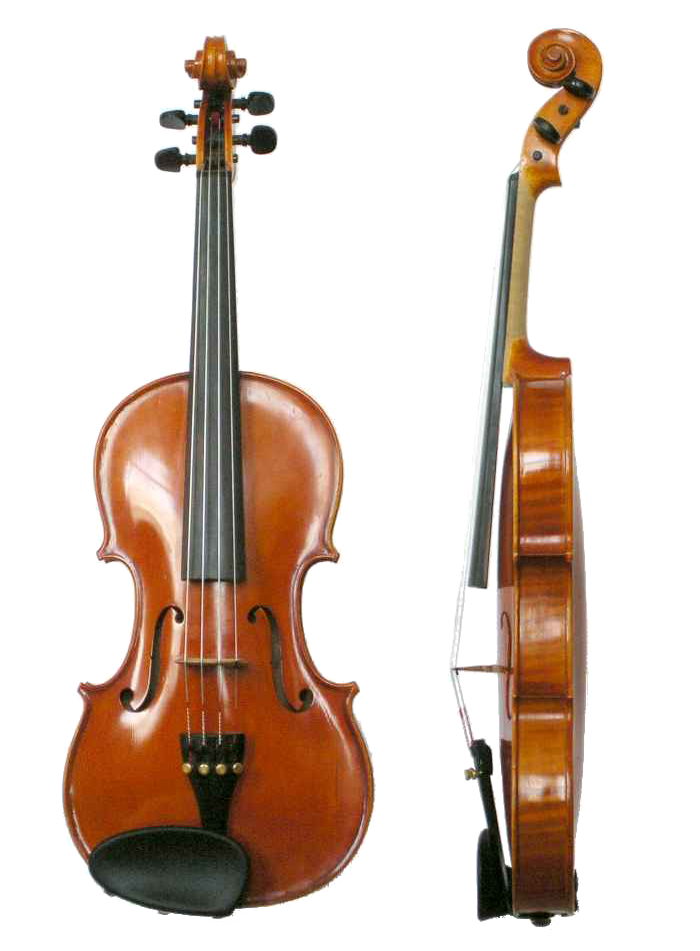
\includegraphics[scale=0.5]{img/22.png}
  \caption {violin}
  \label{fig:violin}
\end{figure}

Podemos ver un ejemplo de un violin en
\emph{\textbf {violín}}~\ref{fig:violin}
